\documentclass[tikz,border=2mm]{standalone}
\usepackage[T1]{fontenc}
\usepackage[utf8]{inputenc}
\usepackage{lmodern}
\usepackage{xcolor}
\usepackage{tikz}
\usetikzlibrary{calc, positioning, arrows.meta, decorations.pathreplacing}

\definecolor{umbruchred}{HTML}{E63946}
\definecolor{umbruchblue}{HTML}{457B9D}
\definecolor{umbruchgray1}{HTML}{333333}
\definecolor{umbruchgray2}{HTML}{666666}
\definecolor{umbruchgray3}{HTML}{999999}
\definecolor{umbruchgray4}{HTML}{E0E0E0}

\begin{document}
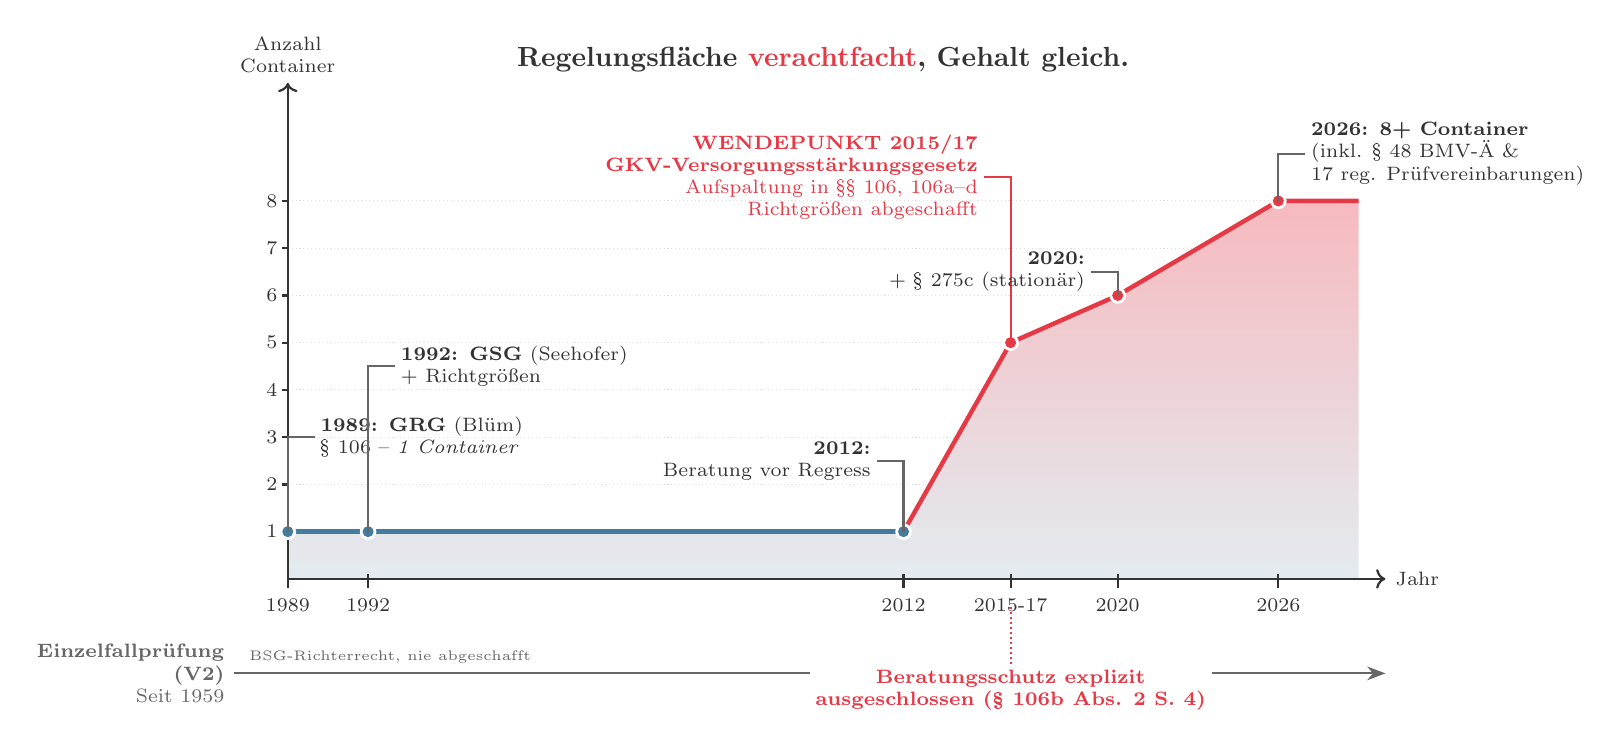
\begin{tikzpicture}[x=0.34cm, y=0.6cm, font=\sffamily\small]

% Background grid
\foreach \y in {1,...,8} {
    \draw[umbruchgray4, densely dotted] (0,\y) -- (40,\y);
}

% Area Chart (Fläche) with vertical gradient reflecting height
\shade[bottom color=umbruchblue!15, top color=umbruchred!35] (0,0) -- (0,1) -- (23,1) -- (27,5) -- (31,6) -- (37,8) -- (40,8) |- (0,0);

% Line outlining the curve (Blue before Wendepunkt, Red starting from Wendepunkt ramp)
\draw[umbruchblue, ultra thick] (0,1) -- (23,1);
\draw[umbruchred, ultra thick] (23,1) -- (27,5) -- (31,6) -- (37,8) -- (40,8);

% X axis
\draw[->, thick, umbruchgray1] (0,0) -- (41,0) node[right, font=\scriptsize] {Jahr};
\draw[->, thick, umbruchgray1] (0,0) -- (0,10.5) node[above, align=center, font=\scriptsize] {Anzahl\\Container};

% Y-axis ticks
\foreach \y in {1,2,3,4,5,6,7,8} {
    \draw[thick, umbruchgray1] (-0.2,\y) -- (0,\y) node[left, font=\scriptsize, umbruchgray1] {\y};
}

% Colors for nodes
\colorlet{col1989}{umbruchblue}
\colorlet{col1992}{umbruchblue}
\colorlet{col2012}{umbruchblue}
\colorlet{col2016}{umbruchred}
\colorlet{col2020}{umbruchred}
\colorlet{col2026}{umbruchred}

% Year Ticks and Data Points
\foreach \x/\y/\v/\col in {0/1989/1/col1989, 3/1992/1/col1992, 23/2012/1/col2012, 27/2015-17/5/col2016, 31/2020/6/col2020, 37/2026/8/col2026} {
    \draw[thick, umbruchgray1] (\x,0.1) -- (\x,-0.2) node[below, font=\scriptsize] {\y};
    \fill[white] (\x,\v) circle (3pt);
    \fill[\col] (\x,\v) circle (2pt);
}

% Callout Styles
\tikzset{
  callout line/.style={draw, umbruchgray2, thick},
  lbl/.style={align=left, font=\scriptsize, umbruchgray1, inner sep=2pt},
  lblR/.style={align=right, font=\scriptsize, umbruchgray1, inner sep=2pt},
  lblC/.style={align=center, font=\scriptsize, umbruchgray1, inner sep=2pt}
}

% -- Annotations --

% 1989
\draw[callout line] (0,1) -- (0, 3) -- (1, 3);
\node[lbl, anchor=west] at (1, 3) {\textbf{1989: GRG} (Blüm)\\§ 106 -- \textit{1 Container}};

% 1992
\draw[callout line] (3,1) -- (3, 4.5) -- (4, 4.5);
\node[lbl, anchor=west] at (4, 4.5) {\textbf{1992: GSG} (Seehofer)\\+ Richtgrößen};

% 2012
\draw[callout line] (23,1) -- (23, 2.5) -- (22, 2.5);
\node[lblR, anchor=east] at (22, 2.5) {\textbf{2012:}\\Beratung vor Regress};

% 2015/17
\draw[callout line, umbruchred, thick] (27,5) -- (27, 8.5) -- (26, 8.5);
\node[lblR, anchor=east, umbruchred] at (26, 8.5) {
    \textbf{WENDEPUNKT 2015/17}\\
    \textbf{GKV-Versorgungsstärkungsgesetz}\\
    Aufspaltung in §§ 106, 106a--d\\
    Richtgrößen abgeschafft
};

% 2020
\draw[callout line] (31,6) -- (31, 6.5) -- (30, 6.5);
\node[lblR, anchor=east] at (30, 6.5) {\textbf{2020:}\\+ § 275c (stationär)};

% 2026
\draw[callout line] (37,8) -- (37, 9) -- (38, 9);
\node[lbl, anchor=west] at (38, 9) {
    \textbf{2026: 8+ Container}\\
    (inkl. § 48 BMV-Ä \&\\
    17 reg. Prüfvereinbarungen)
};

% Kernaussage
\node[align=center, umbruchgray1, font=\normalsize\bfseries] at (20, 11) {Regelungsfläche \textcolor{umbruchred}{verachtfacht}, Gehalt gleich.};

% Lower part: V2 Line Since 1959
\draw[thick, umbruchgray2, -{Stealth}] (-2, -2) -- (41, -2);
\node[anchor=east, align=right, font=\scriptsize, umbruchgray2] at (-2, -2) {\textbf{Einzelfallprüfung}\\\textbf{(V2)}\\Seit 1959};
\node[anchor=south west, align=left, font=\tiny, umbruchgray2] at (-1.8, -2) {
    BSG-Richterrecht, nie abgeschafft
};

% Exclude highlight for V2
\draw[umbruchred, thick, densely dotted] (27, -0.6) -- (27, -1.8);
\node[anchor=north, align=center, font=\scriptsize\bfseries, umbruchred, fill=white, inner sep=2pt] at (27, -1.8) {
    Beratungsschutz explizit\\ausgeschlossen (§ 106b Abs. 2 S. 4)
};

\end{tikzpicture}
\end{document}
